The transitory frequency response of the system and therefore its stable and reliable operation after a perturbation, depends on the inherent characteristics of the power system and the counteraction measurements engaged automatically by the power system. As the share of inverter based generation increases, the more sensible to instability the power system becomes. In this sense the added inverter based fast power reserve must be capable of maintaining transitory frequency value within the allowed limits. 
Two terms commonly found in the literature of power system stability will be used along this section:

\begin{itemize}[leftmargin=*,labelsep=5.8mm]
	\item \textbf{Inertia constant (H)}: It has units of seconds (s) and it is the ratio of the kinetic energy stored in the rotating masses of the generators ($E_k$ in MWs) and its nominal capacity ($S_{nom}$ in MVA).\\
	\item \textbf{Acceleration time constant (T\textsubscript{a})}: It also has the units of seconds (s) but this is the ratio of double the kinetic energy (MWs) and generators nominal power output ($P_{nom}$ in MW).\\
	 Acceleration time constant is a measure of the robustness before disturbances of the system. It could be interpreted as the required time to remove the kinetic energy from the rotating masses of the generators connected in a grid at the rate of the supplied power load. Hence, the higher the time constant, the higher the kinetic energy available. As the share of synchronous generations decreases, this constant decreases proportionally.
\end{itemize}

With $f$ as frequency, $f_0$ as nominal frequency and $\Delta P$ as power imbalance the swing equation can be expressed as follows:
%Equation 3 1
\begin{equation}
	\label{eq:swing}
	\frac{df}{dt}=\dfrac{\Delta P*f_0}{2*H*S_{nom}}=\frac{\Delta P*f_0}{T_a*P_{nom}}=\frac{\Delta P*f_0}{2*E_k}
\end{equation}
%df/dt=(∆P*f_0)/(2*H*S_nom )=(∆P*f_0)/(T_a*P_nom )=(∆P*f_0)/(2*E_k )
In this paper, the inertia constant $ H $ is used for the description of synthetic inertia in wind turbines, whereas the system acceleration constant $ T_a $ is used to express the whole system inertia related to the load in terms of real power.

\subsection{Synthetic Inertia}


Synthetic inertia is one of the new techniques that manufactures and researchers are considering to tackle with the low inertia problem in power systems  [23, 24]. Frequency support through synthetic inertia was considered with the following assumptions [6, 25]:
\begin{enumerate}[leftmargin=*,labelsep=4.9mm]
	\item Power output from synthetic inertia is limited to 10\% of wind turbine nominal power.
	\item Due to mechanical and thermal stresses, the additional power can be delivered only for a maximum time of 10 s.
	\item It is assumed that all wind turbines operate at its maximum power output. The value of 1.5 MW was selected for such purpose.
	\item In order to avoid wind turbine stall, the removed kinetic energy from the blades (injected to the grid in electrical form) it is limited to half [26].

\end{enumerate}

	An adequate control system is needed so the stored energy in the rotating blades can be extracted from the wind turbine. From the expression of power as the derivative of energy stored in the blades \eqref{eq:si}, the rate of energy extracted from the wind turbine can be obtained, considering that the rotational speed changes in time ref.

\begin{equation}
	\label{eq:si}
	P_{pu}(t)=2*H_{wt}*\omega_{pu}(t)*\dfrac{d\omega_{pu}(t)}{dt}
\end{equation}

%Equation 3 4 

Where  $H_{wt}$ is the turbine inertia constant and $\omega_{pu}$ the rotational speed in per unit.\\

\begin{figure}[h]
	\centering
	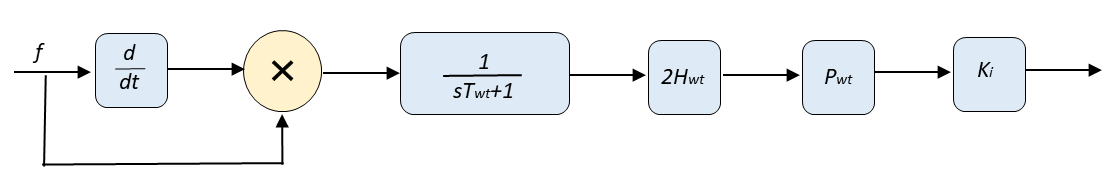
\includegraphics[width=0.6\textwidth]{/method/SI}
	\caption{Representation of equation \eqref{eq:si} in the model. In the figure it can be seen the insertion of a filter at the output of the multiplication block. A constant block $ K_i $ adjusts the initial response in the model. Since equation \eqref{eq:si} is given in pu, the output is multiplied by a constant $ P_{wt} $ representing the rated power of the turbine.}
	\label{fig:synthetic}
\end{figure}





%Equation \eqref{eq:si} was implemented in SIMULINK with the addition of a gain block $K_i$, in order to inject more power from the very beginning of the power imbalance. A filter at the signal entrance was added in order to suppress non desired oscillations on the system [24, 25].\\

%Insert diagram of synthetic inertia here

Typical values for inertia constant of wind turbines are not openly available from the manufacturers to the public. Hence an approximate value was calculated with the utilization of an equation which relates nominal power and inertia constant for wind turbines [27].
\begin{equation}
	\label{eq:wtinertia}
	H_{wt}\approx1.87*P_{nwt}^{0.0597}
\end{equation}
%Equation 3 5: Wind turbine inertia constant as function of the nominal power in MW.
%H_wt≅1.87*P_nwt^0.0597
For a wind turbine with nominal power output of 1.5 MW the value of $ H $ corresponds to 4.37 s [28].
It is assumed that all the wind turbines deliver their nominal power output. A rated rotational speed of 18 rev/min was considered [28]. To avoid the wind turbine to stall, a reduction of 5 rev/min it is allowed by the implementation of the control system. This change of rotational speed equals a change of 3 MWs reduction on kinetic energy out of a total of 6 MWs.

%Table 3 1: Constants for implementation of synthetic inertia.
\begin{table}[h]
	\caption{\label{tb:inertia}: Constants for implementation of synthetic inertia}
	\centering
	%% \tablesize{} %% You can specify the fontsize here, e.g., \tablesize{\footnotesize}. If commented out \small will be used.
	\begin{tabular}{cccc}
		\toprule
		\textbf{T\textsubscript{wt}} 	& \textbf{ H\textsubscript{wt} (s)}	& \textbf{ P\textsubscript{wt} (MW)}  & \textbf{ K\textsubscript{i}} \\
		\midrule
			1	       & 4.37		        &  1.5*$ n_{wt} $\footnote{Number of wind turbines with synthetic inertia control} & 10 \\
		%entry 2		& data			& data\\
		\bottomrule
	\end{tabular}
\end{table}

\subsection{Inverter based fast Power Reserve}


%Figure 3 1 depicts the typical frequency response when a negative power imbalance occurs in a power system. If the imbalance is high enough or the system inertia is too low, the initial RoCoF can lead to frequency %excursions below the UFLS value. The value of RoCoF is brought to zero normally by the action of the primary reserve; equalizing the power imbalance assuming no load frequency dependency. At this time the minimum value %of frequency (frequency nadir) is reached as well.
When a power system is subjected to a negative power imbalance and it is assumed that no load is rejected at UFLS frequency, this continues dropping below 49 Hz. The time at which the system frequency equals the UFLS value is then called critical time. This is the maximum available time for the inverter based reserve to deploy the required power to the system. \\

\begin{figure}[h]
	\centering
	\begin{subfigure}[h]{0.45\textwidth}
		\centering
		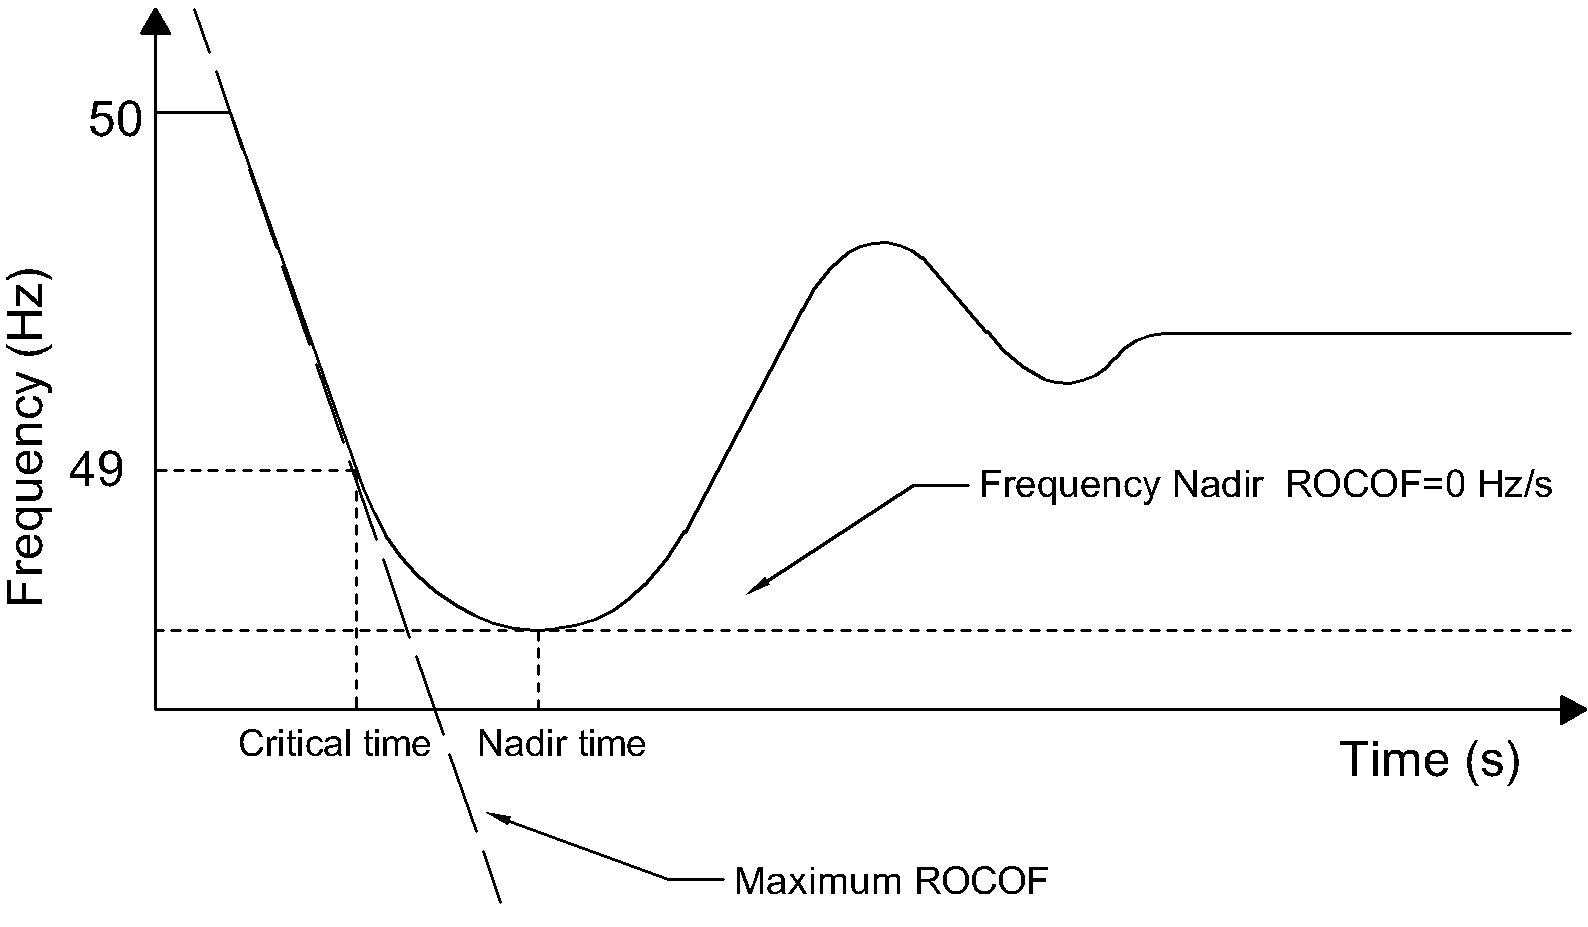
\includegraphics[width=\textwidth]{method/fig1}
		\caption{Typical frequency response leading to UFLS}
		\label{fig:freqresp_before}	
	\end{subfigure}
	\hfill
	\begin{subfigure}[h]{0.45\textwidth}
		\centering
		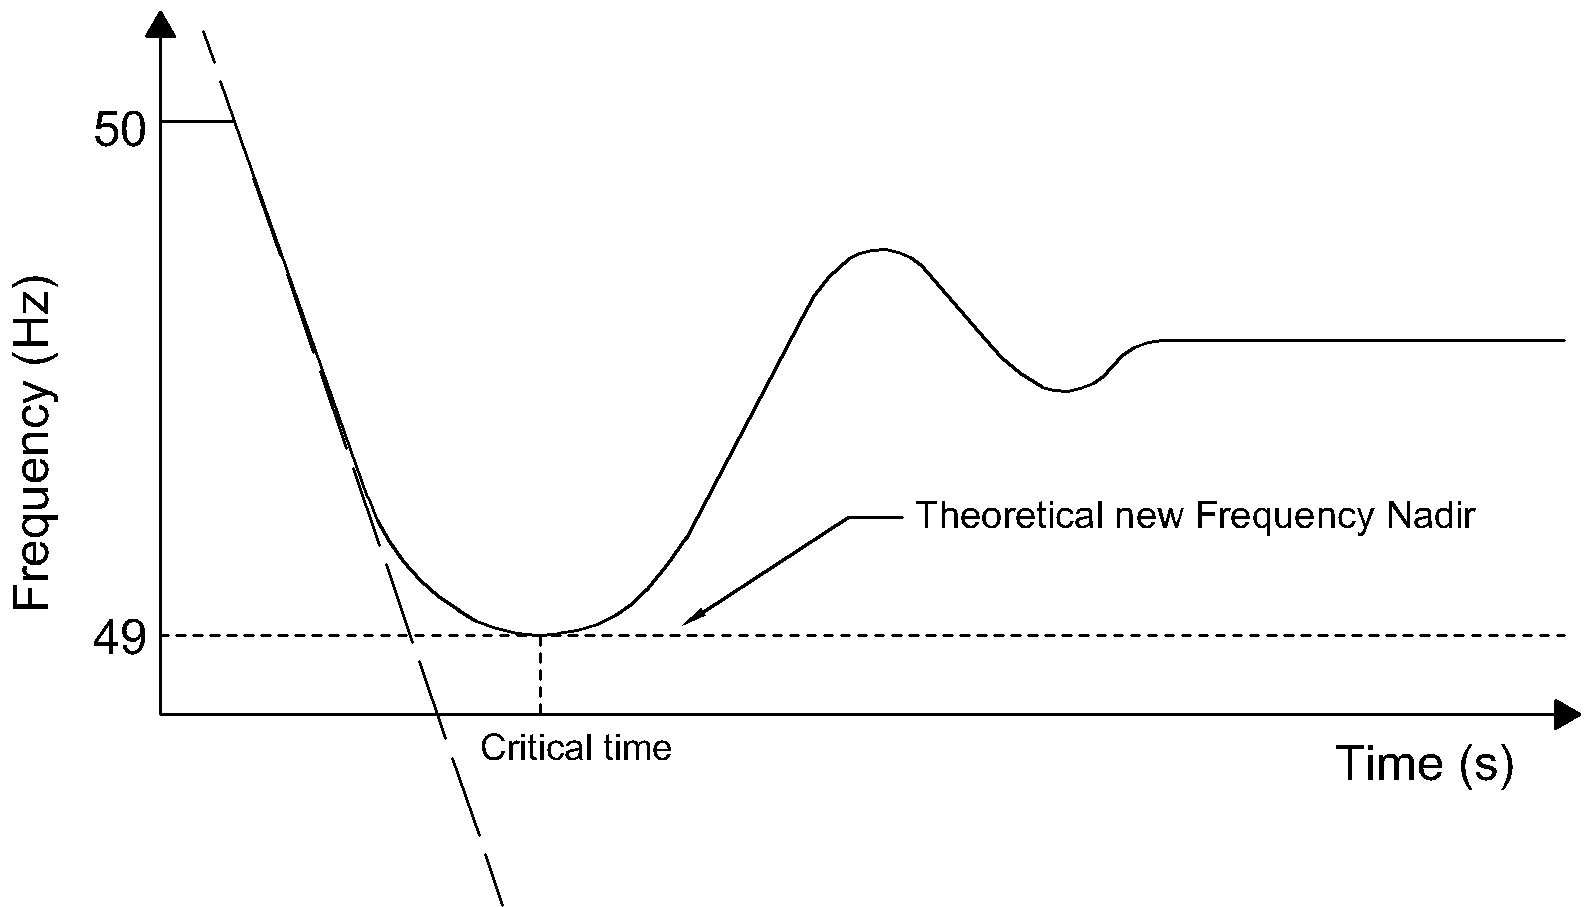
\includegraphics[width=\textwidth]{method/fig2}	
		\caption{Desired frequency response avoiding UFLS}
		\label{fig:freqresp_after}
	\end{subfigure}
	
	
	\caption{In (\textbf{a}) the frequency response goes below the 49 Hz leading to UFLS at the critical time, whereas in (\textbf{b}) the IBFPR is applied avoiding ULFS. In this case the power imbalance is compensated at the critical time by the inverters.}
\end{figure} 

In the critical condition that would lead to load shedding, it is expected from the IBFPR to at least to counteract the RoCoF at the critical time, as illustrated in Figure \ref{fig:freqresp_after}.
Recalling equation \eqref{eq:swing}; it is necessary that the machine’s accelerating power (power imbalance) become zero at the critical time.
\begin{equation}
	\label{eq:powerbalance}
	P_a (t_{cr} )=P_{mech}-P_{elec}+P_{IBFPR}=0
\end{equation} 

Where $ P_a $ is accelerating power, $ P_{mech} $ is mechanical power, $ P_{elec} $ is electrical power load, $ t_{cr} $ is the critical time and $ P_{IBFPR} $ is inverter based fast power reserve.
%Typical primary power reserve response follows the indicated behavior shown in Figure 3 . Conventional turbine governor response is frequency dependent and may not respond linearly. For the estimation of IBFPR it was %assumed a linear power deployment over time until the critical time. Inspecting Equation 3 1; it can be notice that only the power imbalance determines the rate of change in frequency in the system along with the kinetic energy stored in the rotating masses of the generators. For this reason the analysis is focused on the change on mechanical power after the event, ignoring the electrical load and mechanical power in the stable operation before the perturbation.
From the assumption of a linear mechanical power deployment is given from the synchronous machines governors, the rate of change in mechanical power, after a power imbalance $ \Delta P $, is given by $ \Delta P/t_{nadir} $, where $ t_{nadir} $ represents the time at which the frequency nadir occurs. Given the power balance at the critical time, $ t_{cr} $; the IBFPR response must be equal to $ P_{elec}-P_{mech} $, being $ P_{elec} $ equal to $ \Delta P $. %Figure 3  illustrates the behavior of both responses together. The sum of both at critical time counteracts power imbalance.


Substituting $ P_{mech} $ by $ \Delta P* t_{cr} /_{tnadir} $ and $ P_{elec} $ by $ \Delta P $ in \eqref{eq:powerbalance}, the following expression is obtained for the $ P_{IBFPR} $ at time $ t_{cr} $:
%Equation 3 2 

\begin{equation}
	\label{eq:p_at_tcr}
	P_{IBFPR} (t_{cr} )=\Delta P*(1-t_{cr}/t_{nadir} )
\end{equation}
It is assumed that $ P_{IBFPR} $ remains with a constant power output after $ t_{cr} $ long enough to stabilize the system frequency. The result of the previous equation represents the slope of the power output since the inception of the incident until the critical time, which with the implementation of IBFPR, it will be not any longer critical but rather it will be the new desired frequency nadir time.
%Equation 3 3: IBFPR before critical time.
\begin{equation}
	\label{eq:IBFPR}
	P_{IBFPR} (t)=\dfrac{\Delta P*(1-t_{cr}/t_{nadir} )*t}{t_{cr}}
\end{equation}
%P_IBFPR (t)=∆P/t_cr *(1-t_cr/t_nadir )*t

%The positive value of \eqref{eq:IBFPR} represents the injection of fast power response from renewables or storage to counteract frequency drop below of the load shedding frequency setting of 1 Hz below nominal. Nevertheless when there is an over-frequency phenomenon with surplus in generation, the negative value of \eqref{eq:IBFPR} can be taken as the power rate required to limit over-frequency to no more than 1 Hz above nominal. Similarly, critical times would apply for upper and down frequency thresholds.\\  

According to the obtained expression; it can be realized that the desired power response from the inverters depends exclusively on parameters which cannot be directly measured from the grid connection point. In a real situation the values of $\Delta P$, $ t_{nadir} $ and $ t_{cr} $ cannot be known in advance, representing this factors a challenge in the implementation of this ideal power response. Those values are dependent on the grid characteristics, the primary conventional reserve deployment time and the overall system inertia [18]. Thus two main cases are considered for the remaining analysis with the intent of covering a wider range of systems with different characteristics and dimensions.

\subsection{Simulation Cases}

As presented in the previous section, the values of critical time and frequency nadir time depend on the system imbalance and primary reserve deployment time.  In spite of assessing the influence of the grid size and the primary reserve characteristics, two main cases are considered. In both cases is assumed that the initial steady frequency is the nominal 50 Hz.


\begin{itemize}[leftmargin=*,labelsep=5.8mm]
	\item \textbf{Small scale grid case:} For the evaluation of this case typical governor data is considered in a well-known and studied benchmark grid topology as the WSCC model, also known as the IEEE 9 bus model. Synchronous reserve deployment is in the order of a few seconds due to governor response [7, 11].
	\subitem Scenario A - Simplified Model: The power system is represented by an equivalent single machine model in which losses are neglected. It is investigated the critical time for inverters' activation and the required IBFPR is  also determined. Furthermore, the impact of synthetic inertia and the frequency measurement delay in frequency response is analyzed.
	\subitem Scenario B - Extended Model: All the power system components (transmission lines, transformers, exciters and governors of the three generators) and its dynamic characteristics are considered in the IEEE 9 bus model.\\
	\item \textbf{Large scale grid case:} The European grid scale in which all the synchronous machines are modeled and simplified as one single machine, provided with the characteristic expected from the overall system. Synchronous primary reserve deployment is in the order of $ \sim30 $ s [1, 19]. Island frequency response is assumed to be the same that the European response analyzed by ENTSOE ref.
\end{itemize}



\subsection{Simplified IEEE 9 bus Model}
\label{ssec:simpleieee}
%Microgrids can operate connected to the bulk transmission/distribution system or stand alone. In any case
%It is assumed that imbalances could occur due to internal faults when island configuration is considered or islanding from the external system results from a contigency while a considerable amount of power load of the microgrid was being `imported’ or `exported’. For the study of power systems and the increasing interest in stability analysis for DER integration, the IEEE benchmarks represent a widely used option, based on some real data. This is also the case of the IEEE 9 bus model or WSCC (Western System Coordinated Council). The IEEE 9 bus model is a representation of the former western interconnected power system of North America of 1967. For stability and reliability studies, this system has been employed in many publications as study case [20], which allows the comparison of results. Figure 3 3 illustrates grid’s configuration. 
As a first step to evaluate the impact of inverter based generation and power imbalances in the grid, the whole system is simplified as one single generating unit; neglecting all losses in the system (Transformers, transmission lines and generators) with the assumption that the mechanical output of the prime mover is the same than the electrical power output at generator terminals. Table \ref{tb:gridelements} provides a summary of the elements comprising the base model.\\

\begin{table}[h]
	\caption{\label{tb:gridelements}:Elements of the IEEE 9 bus model.}
	\centering
	%% \tablesize{} %% You can specify the fontsize here, e.g., \tablesize{\footnotesize}. If commented out \small will be used.
	\begin{tabular}{ccc}
		\toprule
		\textbf{}	& \textbf{Quantity}\\
		\midrule
		Buses		& 9			\\
		Transformers		& 3			\\
 		Transmission Lines			& 6 \\
		Generators			& 3 \\
 		Load			&  315 MW  \\
		\bottomrule
	\end{tabular}
\end{table}





Figure \ref{fig:ieeesimple} is the block representation of the swing equation \eqref{eq:swing}, it only differs in the fact that blocks representing the inverter based generation have been included. The mechanical power is represented by the output of a steam turbine governor model, which is used to represent the synchronous machine [8]. When equilibrium is lost, the accelerating power is multiply by the transfer function $ 1/(2*H*S) $, where $ H $ is the machine’s inertia constant and $ S $ is the machine’s power rating. From \eqref{eq:swing} this product equals the derivative of frequency, therefore an integrator block is added to obtain the frequency response [7, 21, 22]. A feedback loop is added and an error signal obtained from the reference frequency so the synchronous machine can react as frequency deviates from nominal. \\ 

\begin{figure}[h]
	\centering
	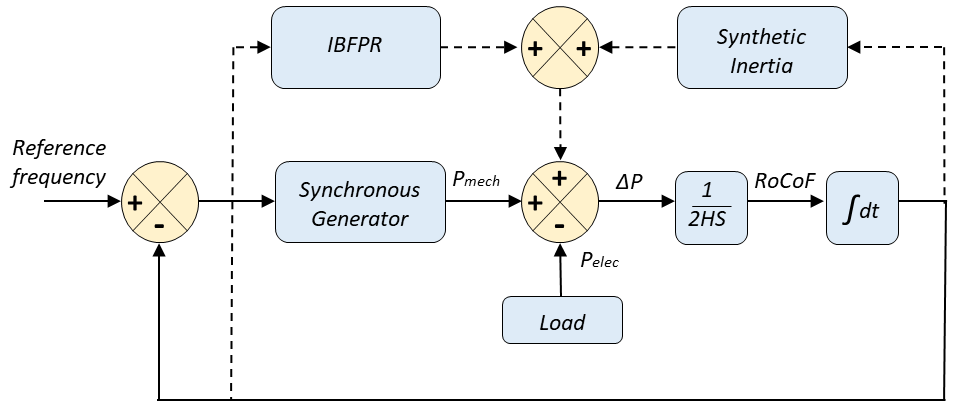
\includegraphics[width=0.6\textwidth]{/method/ieee}
	\caption{Simplified representation of the IEEE 9 bus model. Blocks linked by the solid line represent the conventional swing equation given by \eqref{eq:swing}. Represented with doted lines, the respective frequency signals to the blocks of IBFPR and synthetic inertia, which add power to the system.}
	\label{fig:ieeesimple}
\end{figure}


The values of kinetic energy and time constants of a synchronous machines of 835 MVA were selected to represent the synchronous response, with the load of 315 MW the system acceleration time constant is 14 s [8], which is approximately today’s Europe acceleration constant [1]. This is the base scenario where an 100\% synchronous generation is assumed . For the sake of evaluating the impact of the penetration of inverter based generation; the values of lower capacity generators were selected, diminishing in the sense the total system inertia [8].\\% assuming the compensation of the remaining power by a constant power source representing the inverter based generation, decreasing in this manner the total system acceleration time constant, thus the kinetic energy of the generator. Up to this point, neither synthetic inertia nor frequency support from renewables is considered. Inverter based power output remains constant before, during and after the perturbation. Therefore the system imbalance is covered only by the synchronous equivalent machine.





Even though load imbalances up to 40\% were simulated in each inertia scenario, for estimation of the critical time the power capacity limit of the generators was disregarded. The negative imbalance was simulated by increasing the system load. A block diagram representing the system shown in Figure \ref{fig:ieeesimple} was implemented in SIMULINK with different combinations of power imbalance and system inertia. %With the help of a MATLAB code several simulations were run and the critical and nadir times acquired for each scenario. With the calculated times, the IBFPR to avoid load shedding under each scenario was calculated as given by Equation 3 3 and it is shown in the Results section.
%All the acquired values of critical time, as result from the simulations, are then related with the system RoCoF, so a regression can be performed and link the critical time with system RoCoF.
%For the conditions of the system and the employment of the fitting tool provided by MATLAB, an expression is obtained for critical time as a function of RoCoF.
%For unstable conditions the maximum critical time is 2.7 seconds. Therefore critical time must be lower or equal to that value; calculating in this way that the minimum RoCoF for activation as 0.6143 Hz/s, when the fitting equation obtained from the regression is used.

\subsection{Extended IEEE 9 bus Model}

%It was previously stated that in the first approach, only the total load was considered in the simulations as well as the synchronous generation represented by one single machine and no system losses. 
Since it is desired to compare the results obtained in \ref{ssec:simpleieee} against some model that takes into account the whole system components, losses and dynamics; An  extended representation of the IEEE 9 bus model was implemented in SIMULINK [20]. In this representation, simulations for different values of system inertia and load imbalance were performed, similarly as it was done with the simplified representation of the model. Figure \ref{fig:ieeeext} shows the extended IEEE 9 bus grid architecture with IBG added.\\
\begin{figure}[h]
	\centering
	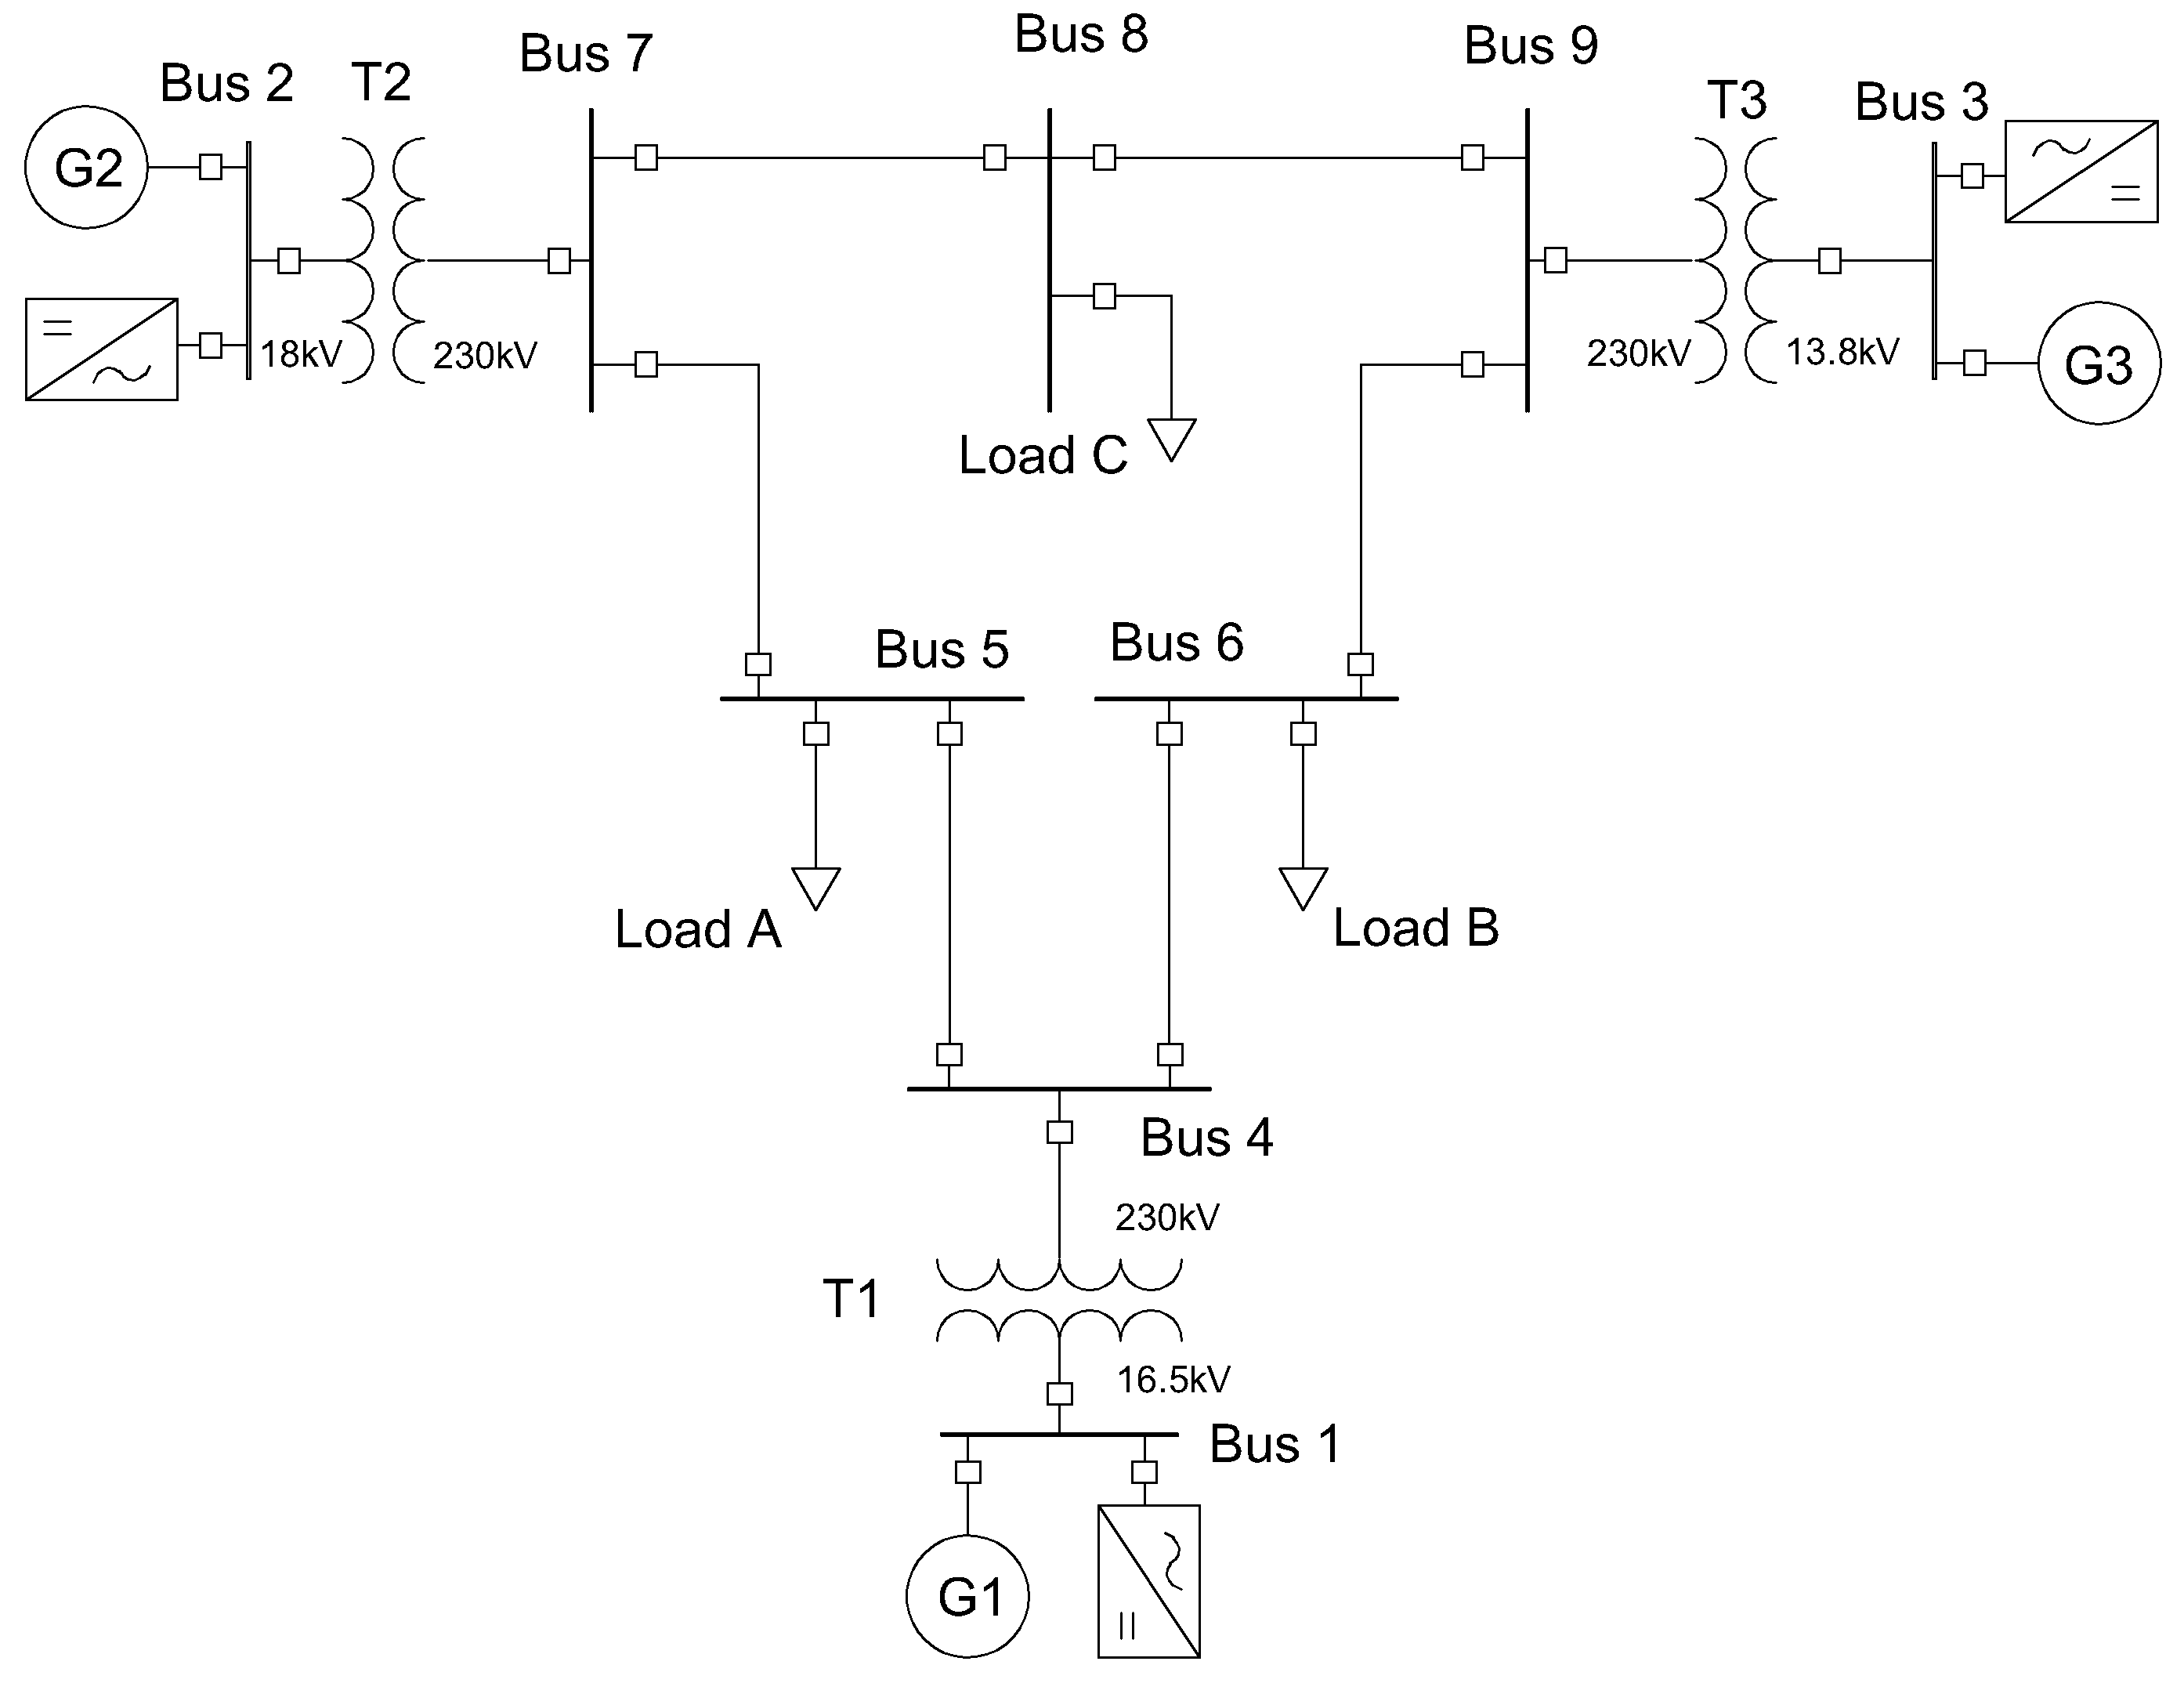
\includegraphics[width=0.5\textwidth]{/method/IEEE_FPRmodel}
	\caption{One line diagram of the IEEE 9 bus model. The inverter based frequency response has been added At the same bus of the generating units.}
	\label{fig:ieeeext}
\end{figure}
In order to evaluate the validity of the equation describing the IBFPR needed to avoid ULFS, the IEEE model was modified with the insertion of ideal controlled power sources blocks, which were set up to inject power into the grid accordingly to the simulated scenario. Therefore, no means of frequency measurement were included and only IBFPR was assessed.
Similarly as it was done in section \ref{ssec:simpleieee}, the total acceleration time constant of the system equals 14 s. Hence the same kinetic energy should be distributed among the three generators' rotating masses in the extended model as in the simplified representation. From \eqref{eq:t_sys} it can be easily calculated that the system kinetic energy with 14 s is 2205 MWs (100\% synchronous generation).
\begin{equation}
	\label{eq:t_sys}
	T_{sys}=(2*E_{k})/P_{load}
\end{equation}
 
Due to the fact that inverter based generation reduces the system kinetic energy; for different levels of inverter based generation,  the generators nominal capacity values were kept constant and the inertia constant of each machine multiplied by the synchronous share factor $ fss $. The total kinetic energy of the system is the summation of all units. In such manner the synchronous generators in the initial state of equilibrium represent both power sources, inverter based plus synchronous.\\
%Equation 3 7
%E_k=2*(H*f_ss)*S
In order to start the simulations in steady state, a load flow calculation of the grid was carried out with the objective of calculating the initial conditions for the exciter and prime mover models. 
Table\ref{tb:initial} summarizes the main values for setting system initial conditions; acquired from the power flow tool provided by SIMSCAPE.


\begin{table}[h]
	\caption{\label{tb:initial}: Steady state initial conditions of the system}
	\centering
	%% \tablesize{} %% You can specify the fontsize here, e.g., \tablesize{\footnotesize}. If commented out \small will be used.
	\begin{tabular}{ccccc}
		\toprule
		\textbf{Bus number}	& \textbf{Bus Type}	& \textbf{Voltage (pu)}& \textbf{Active Power (MW)}& \textbf{Reactive Power (MVAr)}\\
		\midrule
		1		& Slack			& 1.04 $\phase{0^{\circ}} $     &    72.2    & 25.64    \\
		2		& PV			& 1.025 $\phase{9.83^{\circ}} $      & 163      & 8     \\
		3		& PV			& 1.025 $\phase{4.63^{\circ}} $     & 85       &    -9.41 \\
		5		& PQ			& 0.9949 $\phase{-4.42^{\circ}} $       &125       &  50    \\
		6		& PQ			& 1.01211 $\phase{-4.16^{\circ}} $      &   90     &  30   \\
		8		& PQ			& 1.0172 $ \phase{0.17^{\circ}} $       &  100     &   35   \\
		
		\bottomrule
	\end{tabular}
\end{table}


\subsubsection{IBFPR Representation}


The IBFPR was modeled as controlled current sources. These controlled sources inject active power according to the load imbalance and system inertia simulated. The continuous measurement of voltage is required in order to determine the amount of current needed to supply the requested power. The IBFPR will have symmetrical and balanced characteristics. Due to this reason, the magnitude and angle of the current phasor will be obtained from the positive sequence of the measured voltage. From the definition of complex power and voltage symmetrical components in three phase systems \eqref{eq:complex_p}, the positive sequence component of phase voltage and line current are obtained. [21] 

\begin{equation}
\label{eq:complex_p}
S_{3\varphi}^1=3*V_{LN}^1*\bar{I_{L}}^1
\end{equation}

This equation is valid for RMS values of voltage and current; nevertheless the measured voltage values and the sought current values are given in peak values, the equation for power and current become:

\begin{equation}
\label{eq:power_seq}
S_{3\varphi}^1=\dfrac{3*V_{LNpeak}^1*\bar{I_{Lpeak}}^1}{2}
\end{equation}

%In the SIMULINK model the voltage measurement probes are connected at the medium voltage side of the transformes. %Figure 3 12 shows the block diagram implemented to obtain the positive symmetrical component of line voltage and the positive sequence of current that will be provided by the subsystem to meet to needed power from the ramp input depending on the voltage readings. :

 

\begin{equation}
\label{eq:current_seq}
I_{Lpeak}^1=\dfrac{\bar{2*S_{3\varphi}^1}}{3*V_{LNpeak}^1}
\end{equation}
%Equation 3 10
%〖I_Lpeak〗^1=¯(((2*〖S_3ⱷ〗^1)/(3*〖V_LNpeak〗^1 )))
With the help of the \textbf{a} operator ($-0.5+j\sqrt{3}$ or $ 1\phase{120^{\circ}}) $ the values of the positive sequence component of phase voltage can be obtained. \\
From $ V_a +V_b+V_c=0$ and $ V_a^1=\frac{V_a+ aV_b+a^2 V_c}{3} $:
\begin{align*}
	 V_a^1 & =\dfrac{V_a+ aV_b-a^2 V_b-a^2}{3} \\
	& =\dfrac{V_a*(1-a^2)+ aV_b*(1-a)}{3} 
\end{align*}

Since $V_{an}^1=\frac{V_a^1}{\sqrt{3}\phase{30^{\circ}}}$, $\sqrt{3}\phase{30^{\circ}}=1-a^2 $ and $ \sqrt{3}\phase{-30^{\circ}}=1-a $ then after some algebraic manipulation the expression for $ V_{an}^1 $ becomes:

\begin{equation}
	\label{eq:volt_seq}
	V_{an}^1=\dfrac{V_a-a^2 V_b}{3}
\end{equation}

With the obtained expressions  for the positive sequence of phase voltage \eqref{eq:volt_seq} and complex power \eqref{eq:power_seq}, the needed current \eqref{eq:current_seq} to supply the IBFPR related to the measured voltages can be implemented in SIMULINK as depicted in FIGUREXXX. The ramping function will last until the critical time is reached, afterwards, the IBFPR output will remain constant.

\subsection{Large Scale Case: Europe Power System}

Under normal operation ENTSOE has reported values of RoCoF in the range of 5-10 mHz/s for power outages of 1 GW in the current interconnected power system. If an imbalance event of more than 3 GW occurs with depleted primary reserve, extraordinary values of frequency and RoCoF might be reached. After serious disturbances the Continental European Power System has experienced RoCoF between 100 mHz/s and 1 Hz/s. Imbalances of 20\% or more along with RoCoF greater than 1 Hz/s have been determined by experience to be critical [1].
ENTSOE has determined that under the case of the reference scenario (The loss of 3 GW generation with 150 GW load and 2\%/Hz self-regulation) in the interconnected operation, the influence of inverter based generation, and therefore the reduction of system inertia would not jeopardize system stability. Due to the expected increase of non-synchronous generation in the future, international power trade and renewables variability; ENTSOE estates in its future split reference scenario that the power system must be capable of withstanding imbalances greater than 40\% with RoCoF of 2 Hz/s or higher. Under these circumstances the resulting islands must avoid load shedding. Hence, only the split scenario is considered for further analysis.

When considering the system blackout of November 4th 2006, in which four electric islands resulted from the European system split; system blackout due to under frequency was experienced in the so known western area. This island, at the moment of split, had approximately a load of 190 GW (27\% more than the low load scenarioENTSOE ) [29]. For its comparable `size’ and the uncertainty of knowing beforehand the resulting islands after a major contingency, the selected load for simulation was the same as the ENTSOE reference scenario as well as the primary reserve deployment time. To simulate the behavior of the resulting island in the European split scenario; a simplified approach was selected. Similarly as it was done with the simplified block model for the IEEE 9 bus model, in the equivalent European representation all the synchronous generation will be represented by a single machine, which will provide governor response when a perturbation takes place. Additional to the synchronous response, a load response of 2\% was added to the model, which means that for every Hertz reduced or augmented, the load will reduce or increase by a 2\% [1]. \\
 
%Figure 3 15 depicts the results of ENTSOE for the interconnected reference scenario frequency response model. It is intended that the implemented model for the island would perform in a similar way like the ENTSOE model for the same conditions [1].
In order to fit the behavior of the system to the modeled by ENTSOE, an additional block was added the IEEE simplified model in the steam turbine governor; this was done with the intention of adjusting the time response of the primary reserve as much as possible to the desired one. With this approach, the primary power reserve can be easily tuned with the assistance of the Control System Tuner App available in MATLAB. The period of time of utmost interest for analysis is from the inception of the power imbalance and the nadir time. Therefore, the system must perform as similar as possible in this region compared to the ENTSOE reference, whereas after the nadir time, the disparity between responses can be neglected. In the European scale the reserves must be completely deployed within 30 s after the occurrence of the disturbance.  






\subsubsection{System Parameters}

A power system of $ n $ number of synchronous machines is assumed; having each of them a capacity $ S $ in MVA, a nominal power $ P_{nom} $ in MW.
Assuming that each machine operates at a de-load factor $ dl $ of $ P_{nom} $; with an acceleration constant equal to $ T_{nom} $ then the number of machines $ n $, for the load $ P_{syncload} $, served by synchronous machines is:
%Equation 3 12
%n=P_(load_sync)/(P_nom*dl)
\begin{equation}
	n=\dfrac{P_{syncload}}{P_{nom}*dl}
\end{equation}
Then the time acceleration constant of the system $ T_{sys} $ can be obtained as follows:
\begin{align}
	T_{sys} &=\dfrac{\sum_{i=1}^nP_i*T_i}{P_{LOAD}}\nonumber  \\ 
	 &=\dfrac{nP_{nom}*T_i}{P_{LOAD}}\nonumber \\
	&=\dfrac{P_{syncload}*T_{nom}}{P_{LOAD}*dl}\nonumber\\	
		&=\dfrac{Sync share*T_{nom}}{dl} \label{eq:tsyseuro}
\end{align}




In this sense the system time acceleration constant can be calculated with a synchronous share of 100\%, resulting in $ T_{sys}=12.5 $ s  with values of $ T_{nom}=10 $ s [1, 8], and a de-load factor $ dl=0.8 $.
The values of the additional block in the model are set in order to have a step response with 2\% overshoot and a time constant of 8 seconds [22].
Considering only the swing equation, as done in the model, it can be demonstrated that the RoCoF and therefore the frequency response of the system is only dependent on the percentage of load imbalance and the system acceleration time constant.
From the definition of RoCoF as $ \frac{df}{dt}=\frac{\Delta P*f_0}{2*E_k} $ and  $ T_{sys}=\frac{2*E_k}{P_{LOAD}} $ :

\begin{align}
	\dfrac{df}{dt} &=\dfrac{\Delta P*f_0}{P_{LOAD}*T_{sys}} \nonumber\\
	&=\dfrac{\Delta P_{pu}*f_0}{P_{LOAD}*T_{sys}}
	\label{eq:dfdpeuro}
\end{align}
In \eqref{eq:dfdpeuro} the value of $ \Delta P_{pu} $ is the normalized value of power imbalance having as base power the value of load $ P_{LOAD} $. As shown in the equation, when only the swing equation is considered, the frequency response is only dependent on system acceleration constant and the relative value of imbalance. This relative value of imbalance varies during time, depending on load response to change on frequency and the response of primary reserve of the system.


